\subsection{\jc Architecture}
% run in jcvm

% %
% jcvm smaller than jvm because of card limitations
% limited amount of data types and objects allowed
% to give an idea ... numbers
% more space than on cards if supported?
Applets installed on a \jc run in the \jc Virtual machine (JCVM) on the smart card. The hardware is limited and as a result, it is necessary that the JCVM is small in size. Most cards have $1.2$kB of RAM, $32-48$kB ROM and $16$kB EEPROM\cite[Sec. 2.1]{java_card_spec}. To save resources, only a limited number of data types are supported, such as \texttt{short} and optionally integers while others such as \texttt{string} and \texttt{double} are not. If \texttt{string} and \texttt{double} were to be supported, code for performing string manipulation and floating point arithmetic would have to be included, which would take up valuable space.\\\\
% %
% transactions and card tear
The \jc does not have its own power supply and applets must be protected from tears - an unexpected loss of power when a card is removed from a terminal. To handle this a transaction mechanism is provided, which allows a region of code to be atomically executed. If a tear occurs while an applet is executing in this region, operations performed by it are rolled back. This is useful in cases such as a credit card withdrawal process. If a card tear occurs after an internal balance counter is decremented, but before the withdrawal is registered, someone could potentially purchase items without actually paying. If the payment specific code region was protected by the transaction mechanism, the tear would have no effect.\\\\
%
%
The JCVM runs on top of the operating system, as illustrated in \cref{fig:architecture},
% jcvm supports dialect of java byte code
and supports a dialect of Java bytecode.
% jc framework:
% jc specific interfaces and classes, e.g.....
% vendor specific:
% specific used by banking 
On top of the JCVM, there is a final layer on top of which applets reside. The layer contains vendor and industry extensions, such as functionality used in the banking industry.\\\\
% %
% feature not in java: firewall:
%     multiple apps in same memory, separation needed for security, address space, sharable interface to use objects from others, each object has owner, accept request context switch, result returned
The JCVM offers features not found in Java virtual machines, such as a firewall separating the applets' memory. Since multiple applets reside side by side on the \jc, it is vital to protect each applet's memory from other applets. If this was not the case, another applet could freely access and alter the memory of another applet, affecting its behaviour. If an applet needs an object from another, it can implement a shareable interface to expose selected objects. If the request is granted, the JCVM will perform a context switch, and the applet in which the object is residing will run the requested operation on the object. After the operation completes, the result is returned to the requesting applet.

\begin{figure}[H]
\centering
%% Creator: Inkscape 0.91_64bit, www.inkscape.org
%% PDF/EPS/PS + LaTeX output extension by Johan Engelen, 2010
%% Accompanies image file 'architecture.pdf' (pdf, eps, ps)
%%
%% To include the image in your LaTeX document, write
%%   \input{<filename>.pdf_tex}
%%  instead of
%%   \includegraphics{<filename>.pdf}
%% To scale the image, write
%%   \def\svgwidth{<desired width>}
%%   \input{<filename>.pdf_tex}
%%  instead of
%%   \includegraphics[width=<desired width>]{<filename>.pdf}
%%
%% Images with a different path to the parent latex file can
%% be accessed with the `import' package (which may need to be
%% installed) using
%%   \usepackage{import}
%% in the preamble, and then including the image with
%%   \import{<path to file>}{<filename>.pdf_tex}
%% Alternatively, one can specify
%%   \graphicspath{{<path to file>/}}
%% 
%% For more information, please see info/svg-inkscape on CTAN:
%%   http://tug.ctan.org/tex-archive/info/svg-inkscape
%%
\begingroup%
  \makeatletter%
  \providecommand\color[2][]{%
    \errmessage{(Inkscape) Color is used for the text in Inkscape, but the package 'color.sty' is not loaded}%
    \renewcommand\color[2][]{}%
  }%
  \providecommand\transparent[1]{%
    \errmessage{(Inkscape) Transparency is used (non-zero) for the text in Inkscape, but the package 'transparent.sty' is not loaded}%
    \renewcommand\transparent[1]{}%
  }%
  \providecommand\rotatebox[2]{#2}%
  \ifx\svgwidth\undefined%
    \setlength{\unitlength}{153.60819396bp}%
    \ifx\svgscale\undefined%
      \relax%
    \else%
      \setlength{\unitlength}{\unitlength * \real{\svgscale}}%
    \fi%
  \else%
    \setlength{\unitlength}{\svgwidth}%
  \fi%
  \global\let\svgwidth\undefined%
  \global\let\svgscale\undefined%
  \makeatother%
  \begin{picture}(1,0.99741984)%
    \put(0,0){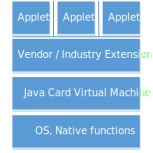
\includegraphics[width=\unitlength,page=1]{architecture.pdf}}%
    \put(0.22925243,0.12061873){\color[rgb]{0.99607843,1,1}\makebox(0,0)[lb]{\footnotesize{OS, Native functions}}}%
    \put(0,0){\includegraphics[width=\unitlength,page=2]{architecture.pdf}}%
    \put(0.15458204,0.3697392){\color[rgb]{0.99607843,1,1}\makebox(0,0)[lb]{\footnotesize{Java Card Virtual Machine}}}%
    \put(0,0){\includegraphics[width=\unitlength,page=3]{architecture.pdf}}%
    \put(0.11513108,0.61886618){\color[rgb]{0.99607843,1,1}\makebox(0,0)[lb]{\footnotesize{Vendor / Industry Extensions}}}%
    \put(0,0){\includegraphics[width=\unitlength,page=4]{architecture.pdf}}%
    \put(0.11487068,0.86337752){\color[rgb]{0.99607843,1,1}\makebox(0,0)[lb]{\footnotesize{Applet}}}%
    \put(0,0){\includegraphics[width=\unitlength,page=5]{architecture.pdf}}%
    \put(0.41012794,0.86337752){\color[rgb]{0.99607843,1,1}\makebox(0,0)[lb]{\footnotesize{Applet}}}%
    \put(0,0){\includegraphics[width=\unitlength,page=6]{architecture.pdf}}%
    \put(0.70539171,0.86337752){\color[rgb]{0.99607843,1,1}\makebox(0,0)[lb]{\footnotesize{Applet}}}%
    \put(0,0){\includegraphics[width=\unitlength,page=7]{architecture.pdf}}%
  \end{picture}%
\endgroup%

\caption{The \jc architectural layers.}
\label{fig:architecture}
\end{figure}